\documentclass{beamer}

\usepackage{amssymb}
\usepackage{fancyvrb}
\usepackage{stmaryrd}
\usepackage{graphicx}
\usefonttheme{serif}


\newcommand{\Nat}{\mathbb{N}}

\title{Natural Language Processing}%\texorpdfstring{$\mathbb{N}$}}
\subtitle{\blueit{Data Science, Spring 2021}}
\date{March 22\textsuperscript{nd}, 2021}

\usetheme{jmct}

\usepackage{calc}

\newcommand{\textover}[3][l]{%
 % #1 is the alignment, default l
 % #2 is the text to be printed
 % #3 is the text for setting the width
 \makebox[\widthof{#3}][#1]{#2}%
 }

\newcommand{\blueit}[1]{%
  {\color{dark-lucid-blue}#1}%
}
\newcommand{\blueite}[1]{%
  \blueit{\emph{#1}}%
}


\newcommand{\myquote}[3]{
  ``#1''
  \vspace{3pt}
  \hrule
  \begin{flushright}
  --- \blueit{\emph{#2}}, \emph{#3}
  \end{flushright}
}

\begin{document}
	\frame {
		\titlepage
	}

%%%%%%%%%%%%%%%%%%%%%%%%%%%%%%%%%%%%%%%% 
%%% Intro
%%%%%%%%%%%%%%%%%%%%%%%%%%%%%%%%%%%%%%%% 

  \frame{
    \frametitle{Before we start...}
      \begin{enumerate}
        \item<2 -> Our mod of the day.
        \item<3 -> Project 1
        \item<4 -> Project 2
        \item<5 -> Midterm
      \end{enumerate}
  }

  \frame{
    \frametitle{Our moderator}
      \begin{enumerate}
        \item<2 -> Julian!
      \end{enumerate}
  }


  \frame{
    \frametitle{Project 1}
      \begin{enumerate}
        \item<2 -> Grading is almost done, I will be posting official mid-semester grades.
        \item<3 -> Regrades are case-by-case. I mostly defer to the TAs so there must be a very compelling issue.
      \end{enumerate}
  }

  \frame{
    \frametitle{Project 2}
      \begin{enumerate}
        \item<2 -> You can use SQL \emph{and} Pandas, it doesn't have to all be SQL (might be impossible?)
        \item<3 -> Plots: \begin{enumerate}
                            \item<4 -> You don't need $N$-plots for $N$ distributions!
                            \item<5 -> Look up box-and-whisker plots.
                          \end{enumerate}
        \item<6 -> Nothing will be accepted after 11:59pm EDT\footnote{Notice the timezone}
      \end{enumerate}
  }

  \frame{
    \frametitle{Midterm}
      \begin{enumerate}
        \item<2 -> Like the quizzes, but significantly more difficult.
        \item<3 -> Last semester's exam is up on the website.
      \end{enumerate}
  }


%%%%%%%%%%%%%%%%%%%%%%%%%%%%%%%%%%%%%%%% 
%%% Part 1
%%%%%%%%%%%%%%%%%%%%%%%%%%%%%%%%%%%%%%%% 

  \begin{frame}
  \centering
    {\fontsize{120}{88} Part I: What.}
  \end{frame}

  \frame{
    \frametitle{Natural Language Processing}
      What is it?
      \begin{enumerate}
        \item<2 -> `Understanding' text
        \item<3 -> Analyzing text
        \item<4 -> Translating text
        \item<5 -> and more!
      \end{enumerate}
  }

  \frame{
    \frametitle{In the olden days:}
      Computation was very expensive, so computationally cheap methods were preferred 
      \begin{enumerate}
        \item<2 -> Dictionary lookup for translation: replace a word in one language with it's `equivalent' in another language.
        \item<3 -> This didn't get very far.
        \item<4 -> Between the 1930's and the 1980's, not much work was done on mechanical translation
      \end{enumerate}
  }

  \frame{
    \frametitle{NLP more generally}
      Two main schools of thought:
      \begin{enumerate}
        \item<2 -> Rule + Grammar-based methods
        \item<3 -> Statistical methods
      \end{enumerate}
      \onslide<4>{These two schools of thought go up and down in popularity.}
  }

 \frame{
  \frametitle{Rule and Grammar-based methods}
    Let's use linguistics to \blueit{formally reason} about language.
      \begin{enumerate}
        \item<2-10> Phonetics
        \item<3-10> Phonology
        \item<4-10> Morphology
        \item<5-10> Syntax
        \item<6-10> Semantics
        \item<7-10> Pragmatics
        \item<8-10> Discourse analysis
        \item<9-10> Stylistics
        \item<10-10> Semiotics
      \end{enumerate}
      \onslide<11>{Sounds complicated... what if we just didn't do that?}
  }

  \frame{
    \frametitle{Statistical Methods}
      Cynically: Through it at some ML techniques and see what happens.
      \begin{enumerate}
        \item<2 -> Decisions tress to automatically learn rules automatically
        \item<3 -> Hidden Markov Models (HMM) for parts-of-speech tagging
        \item<4 -> (Un)supervised learning of language models (this is the hotness)
        \item<5 -> We will discuss some of these techniques in the Machine Learning part of the semester.
      \end{enumerate}
      \onslide<4>{These two schools of thought go up and down in popularity.}
  }

  \frame{
    \frametitle{These methods reflect our biases:}
      \begin{figure}
        
\includegraphics[width=0.75\textwidth]{figs/hungarian.png}
      \end{figure}
  }

  \frame{
    \frametitle{These methods reflect our biases:}
      \begin{figure}
        
\includegraphics[height=\textheight]{figs/turkish.png}
      \end{figure}
  }

  \begin{frame}
  \centering
    {\fontsize{120}{88} Part II: Why.}
  \end{frame}

  \frame{
    \frametitle{Must be nice...}
      Some data scientists have it easy: their data is already in a machine friendly format (HTML/SQL Database/etc). But what about...
      \begin{enumerate}
        \item<2 -> Facebook posts
        \item<3 -> Product reviews
        \item<4 -> data dumps (Panama Papers, wikileaks, etc.)
        \item<5 -> Can you think of other examples?
        \item<6 -> We want this data to be useful too!
      \end{enumerate}
  }

  \begin{frame}
  \centering
    {\fontsize{120}{88} Part III: How.}
  \end{frame}

  \frame{
    \frametitle{`Understanding' is hard}
    ``One morning I shot an elephant in my pajamas.''
    \onslide<2 ->{
      \begin{figure}
        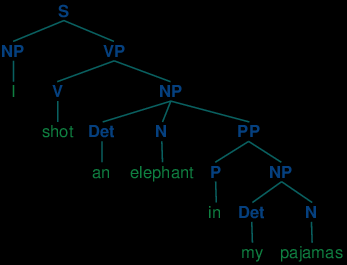
\includegraphics[width=0.5\textwidth]{figs/parse-tree.png}
      \end{figure}}
    \onslide<3 ->{``How he got in my pajamas, I'll never know''}
  }

  \frame{
    \frametitle{`Understanding' is really hard}
    Winograd Schema Challenge:

    ``The city \blueit{councilmen} refused the \blueit{demonstrators} a permit
      because \blueit{they} [\emph{feared}/\emph{advocated}] violence.''
  }

  \frame{
    \frametitle{Sentiment}

    Understanding language directly is very hard. Perhaps understanding \blueit{sentiment} is less hard?

    \onslide<2>{``I bought this product and I use it, but I wouldn't recommend it to my worst enemy''}


    \onslide<3>{``It might seem like this movie is bad, but once you get past the cheesy acting I rather enjoyed it''}
  }

  \frame{
    \frametitle{Summary}

    Summaries are also possible: SMMRY an algorithm for mechanical summaries

  }


%%%%%%%%%%%%%%%%%%%%%%%%%%%%%%%%%%%%%%%% 
%%% Conclusion
%%%%%%%%%%%%%%%%%%%%%%%%%%%%%%%%%%%%%%%% 

  \frame{
    \frametitle{Thanks for your time!}

     :) 
  }


\end{document}
